\documentclass[11pt,oneside,openany]{book}

\usepackage[a4paper,margin=25mm]{geometry}
\usepackage{cscover}
\usepackage[dvipdfmx]{graphicx}
\usepackage[nobreak]{cite}
\usepackage[a4paper,dvipdfmx,pdfdisplaydoctitle=true,%
    bookmarks=true,bookmarksnumbered=true,bookmarkstype=toc,bookmarksopen=true,%
    pdftitle={A Study on Thesis Formats},%
    pdfauthor={Taro Tokodai}%
    ]{hyperref}

\renewcommand{\bibname}{References}
\pagestyle{plain}

\thesistype{Independent Research Project Report:\\Bachelor's Thesis}
\title{A Study on\\Thesis Formats}
\author{Taro Tokodai}
\studentid{17B00000}
\affiliation{%
  Department of Computer Science\\
  School of Computing\\
  Tokyo Institute of Technology}
\date{January, 2021}

\supervisorname{Supervisor:}
\supervisor{Ichiro Joho}
%\dsupervisorname{Deputy Supervisor:}
%\dsupervisor{Jiro Kogaku}

\begin{document}

\frontmatter
\maketitle

\chapter{Abstract}
Single column, unlimited number of pages.

\tableofcontents
\listoffigures
\listoftables

%%%%%%%%%%%%%%%%%%%%%%%%%%%%%%%%%%%%%%%%%%%%%%%%%%

\mainmatter
\chapter{Introduction}
I introduce a sample of how to write a thesis\cite{tokodai-xyz2015}.

\section{Sample}
The followings are samples.
I assume an $n$-dimensional hypersphere shown in Eq.~(\ref{eq:hs}).
In case of $n = 3$, the shape is like in Figure~\ref{fig:hs}.
\begin{equation}
  r^2 = \sum_{k=1}^{n} x_k^2 \label{eq:hs}
\end{equation}
\begin{figure}[htb]
  \centering
  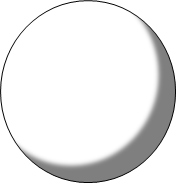
\includegraphics[scale=0.5]{fig/sample.png}
  \caption{A sphere where $n=3$.}\label{fig:hs}
\end{figure}

According to Table~\ref{tab:sample}, it has four elements $(a, b, c, d)$.
\begin{table}[htb]
  \centering
  \caption{Elements}\label{tab:sample}
  \begin{tabular}{|c|r|}
    \hline
    $a$ & $b$ \\ \hline
    $c$ & $d$ \\ \hline
  \end{tabular}
\end{table}

%%%%%%%%%%%%%%%%%%%%%%%%%%%%%%%%%%%%%%%%%%%%%%%%%%

\chapter{Conclusion}
The conclusion should be concise and comprehensive.

%%%%%%%%%%%%%%%%%%%%%%%%%%%%%%%%%%%%%%%%%%%%%%%%%%

\appendix
\chapter{Proof of Theorem 1}
Appendices can be added.

%%%%%%%%%%%%%%%%%%%%%%%%%%%%%%%%%%%%%%%%%%%%%%%%%%

\backmatter
\chapter{Acknowledgment}
Thank you.

%%%%%%%%%%%%%%%%%%%%%%%%%%%%%%%%%%%%%%%%%%%%%%%%%%

\bibliographystyle{plain}
\bibliography{references-e}
%\begin{thebibliography}{99}
%  \bibitem{tokodai-xyz2015} Taro Tokodai. How to write a good thesis. \textit{Journal of XYZ}, 3(4):15--34, 2015.
%\end{thebibliography}

\end{document}
